\def\H{0.3\textwidth}
\def\W{\textwidth}

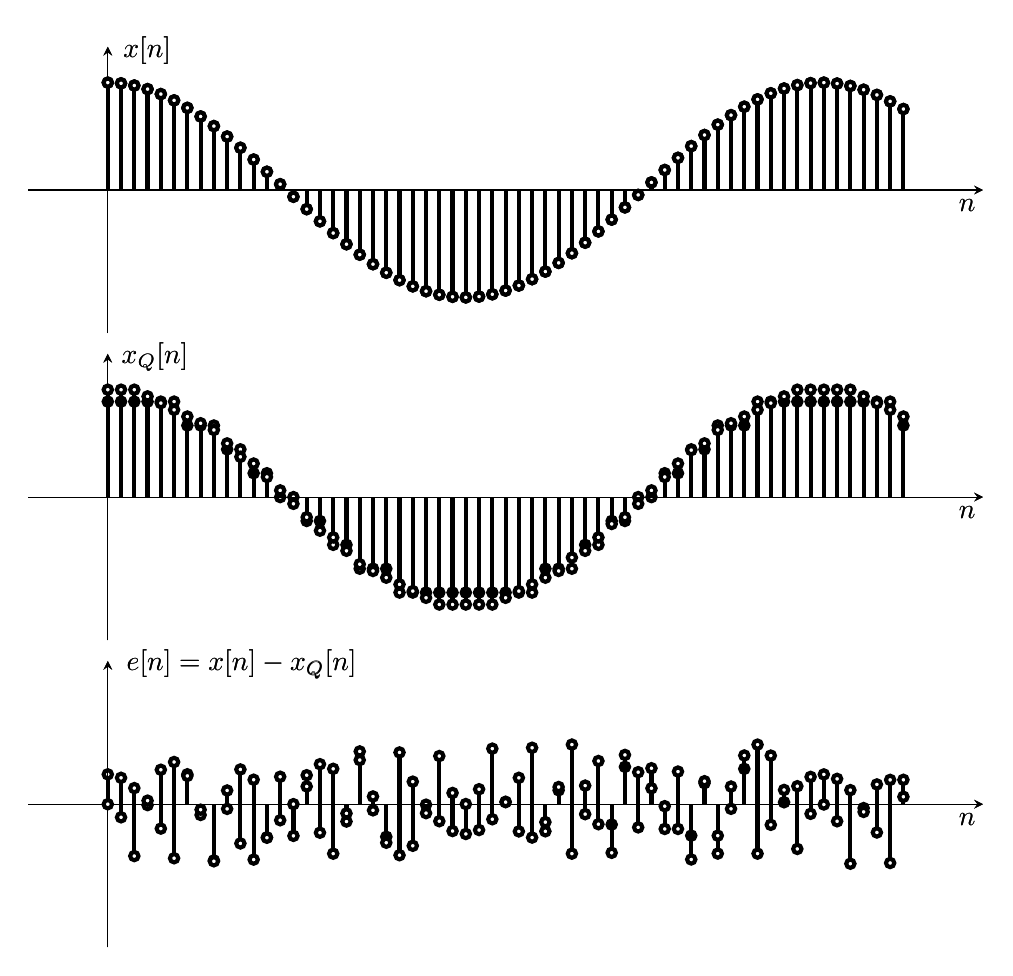
\begin{tikzpicture}
\onslide<1-3|handout:1>{
\begin{axis}[
name=plot1,
axis lines*=middle,
enlargelimits = true,
width=\W,
height=\H,
clip=true,
scale only axis,
axis line style={->,>=stealth},
xlabel={ $n$},
ylabel={ $x[n]$},
every axis x label/.style={
	at={(ticklabel* cs:1)},
	xshift=-0.2cm,
	anchor=north,
},
every axis y label/.style={
	at={(ticklabel* cs:1)},
	xshift=0.5cm,
	yshift=-0.35cm,
	anchor=south,
},
every outer x axis line/.append style={white!15!black},
every x tick label/.append style={font=\color{white!15!black}},
xmin=0.00, xmax=7.00,
ymin=-5.00, ymax=5.00,
ytick=\empty,
xtick=\empty,
yticklabel=\empty,
xmajorgrids,
ymajorgrids,
every outer y axis line/.append style={white!15!black},
every y tick label/.append style={font=\color{white!15!black}},
legend style={draw=white!15!black,fill=white,legend cell align=left}]
\addplot [ycomb, black, mark=*, mark options={scale=0.75, fill=white}, line width=1.5pt, domain=0:7, samples=61, forget plot] {4.5*cos(deg(x))};
\end{axis}
}

\onslide<2-3|handout:1>{
	\begin{axis}[
		name=plot2,
		at=(plot1.below south east), anchor=above north east,
		axis lines*=middle,
		enlargelimits = true,
		width=\W,
		height=\H,
		clip=true,
		scale only axis,
		axis line style={->,>=stealth},
		xlabel={ $n$},
		ylabel={ $x_Q[n]$},
		every axis x label/.style={
			at={(ticklabel* cs:1)},
			xshift=-0.2cm,
			anchor=north,
		},
		every axis y label/.style={
			at={(ticklabel* cs:1)},
			xshift=0.6cm,
			yshift=-0.35cm,
			anchor=south,
		},
		every outer x axis line/.append style={white!15!black},
		every x tick label/.append style={font=\color{white!15!black}},
		xmin=0.00, xmax=7.00,
		ymin=-5.00, ymax=5.00,
		ytick=\empty,
		xtick=\empty,
		yticklabel=\empty,
		xmajorgrids,
		ymajorgrids,
		every outer y axis line/.append style={white!15!black},
		every y tick label/.append style={font=\color{white!15!black}},
		legend style={draw=white!15!black,fill=white,legend cell align=left}]
		\addplot [ycomb, black, mark=*, mark options={scale=0.75, fill=white}, line width=1.5pt, domain=0:7, samples=61, forget plot] {round(4.25*cos(deg(x)))};
	\end{axis}
}

\onslide<3|handout:1>{
	\begin{axis}[
	name=plot3,
	at=(plot2.below south east), anchor=above north east,
	axis lines*=middle,
	enlargelimits = true,
	width=\W,
	height=\H,
	clip=true,
	scale only axis,
	axis line style={->,>=stealth},
	xlabel={ $n$},
	ylabel={ $e[n] = x[n] - x_Q[n]$},
	every axis x label/.style={
		at={(ticklabel* cs:1)},
		xshift=-0.2cm,
		anchor=north,
	},
	every axis y label/.style={
		at={(ticklabel* cs:1)},
		xshift=1.7cm,
		yshift=-0.35cm,
		anchor=south,
	},
	every outer x axis line/.append style={white!15!black},
	every x tick label/.append style={font=\color{white!15!black}},
	xmin=0.00, xmax=7.00,
	ymin=-1.00, ymax=1.00,
	ytick=\empty,
	xtick=\empty,
	yticklabel=\empty,
	xmajorgrids,
	ymajorgrids,
	every outer y axis line/.append style={white!15!black},
	every y tick label/.append style={font=\color{white!15!black}},
	legend style={draw=white!15!black,fill=white,legend cell align=left}]
	\addplot [ycomb, black, mark=*, mark options={scale=0.75, fill=white}, line width=1.5pt, domain=0:7, samples=61, forget plot] {4.25*cos(deg(x)) - round(4.25*cos(deg(x)))};
	\end{axis}
}

%% 8-bit quantizer
\onslide<4-|handout:2>{
	\begin{axis}[
	name=plot1,
	axis lines*=middle,
	enlargelimits = true,
	width=\W,
	height=\H,
	clip=true,
	scale only axis,
	axis line style={->,>=stealth},
	xlabel={ $n$},
	ylabel={ $x[n]$},
	every axis x label/.style={
		at={(ticklabel* cs:1)},
		xshift=-0.2cm,
		anchor=north,
	},
	every axis y label/.style={
		at={(ticklabel* cs:1)},
		xshift=0.5cm,
		yshift=-0.35cm,
		anchor=south,
	},
	every outer x axis line/.append style={white!15!black},
	every x tick label/.append style={font=\color{white!15!black}},
	xmin=0.00, xmax=7.00,
	ymin=-17.7778, ymax=17.7778,
	ytick=\empty,
	xtick=\empty,
	yticklabel=\empty,
	xmajorgrids,
	ymajorgrids,
	every outer y axis line/.append style={white!15!black},
	every y tick label/.append style={font=\color{white!15!black}},
	legend style={draw=white!15!black,fill=white,legend cell align=left}]
	\addplot [ycomb, black, mark=*, mark options={scale=0.75, fill=white}, line width=1.5pt, domain=0:7, samples=61, forget plot] {16*cos(deg(x))};
	\end{axis}
}

\onslide<5-|handout:2>{
	\begin{axis}[
	name=plot2,
	at=(plot1.below south east), anchor=above north east,
	axis lines*=middle,
	enlargelimits = true,
	width=\W,
	height=\H,
	clip=true,
	scale only axis,
	axis line style={->,>=stealth},
	xlabel={ $n$},
	ylabel={ $x_Q[n]$},
	every axis x label/.style={
		at={(ticklabel* cs:1)},
		xshift=-0.2cm,
		anchor=north,
	},
	every axis y label/.style={
		at={(ticklabel* cs:1)},
		xshift=0.6cm,
		yshift=-0.35cm,
		anchor=south,
	},
	every outer x axis line/.append style={white!15!black},
	every x tick label/.append style={font=\color{white!15!black}},
	xmin=0.00, xmax=7.00,
	ymin=-17.7778, ymax=17.7778,
	ytick=\empty,
	xtick=\empty,
	yticklabel=\empty,
	xmajorgrids,
	ymajorgrids,
	every outer y axis line/.append style={white!15!black},
	every y tick label/.append style={font=\color{white!15!black}},
	legend style={draw=white!15!black,fill=white,legend cell align=left}]
	\addplot [ycomb, black, mark=*, mark options={scale=0.75, fill=white}, line width=1.5pt, domain=0:7, samples=61, forget plot] {round(16*cos(deg(x)))};
	\end{axis}
}

\onslide<6-|handout:2>{
	\begin{axis}[
	name=plot3,
	at=(plot2.below south east), anchor=above north east,
	axis lines*=middle,
	enlargelimits = true,
	width=\W,
	height=\H,
	clip=true,
	scale only axis,
	axis line style={->,>=stealth},
	xlabel={ $n$},
	ylabel={ $e[n] = x[n] - x_Q[n]$},
	every axis x label/.style={
		at={(ticklabel* cs:1)},
		xshift=-0.2cm,
		anchor=north,
	},
	every axis y label/.style={
		at={(ticklabel* cs:1)},
		xshift=1.7cm,
		yshift=-0.35cm,
		anchor=south,
	},
	every outer x axis line/.append style={white!15!black},
	every x tick label/.append style={font=\color{white!15!black}},
	xmin=0.00, xmax=7.00,
	ymin=-1.00, ymax=1.00,
	ytick=\empty,
	xtick=\empty,
	yticklabel=\empty,
	xmajorgrids,
	ymajorgrids,
	every outer y axis line/.append style={white!15!black},
	every y tick label/.append style={font=\color{white!15!black}},
	legend style={draw=white!15!black,fill=white,legend cell align=left}]
	\addplot [ycomb, black, mark=*, mark options={scale=0.75, fill=white}, line width=1.5pt, domain=0:7, samples=61, forget plot] {16*cos(deg(x)) - round(16*cos(deg(x)))};
	\end{axis}
}
\end{tikzpicture}